%
% File acl2019.tex
%
%% Based on the style files for ACL 2018, NAACL 2018/19, which were
%% Based on the style files for ACL-2015, with some improvements
%%  taken from the NAACL-2016 style
%% Based on the style files for ACL-2014, which were, in turn,
%% based on ACL-2013, ACL-2012, ACL-2011, ACL-2010, ACL-IJCNLP-2009,
%% EACL-2009, IJCNLP-2008...
%% Based on the style files for EACL 2006 by 
%%e.agirre@ehu.es or Sergi.Balari@uab.es
%% and that of ACL 08 by Joakim Nivre and Noah Smith

\documentclass[11pt,a4paper]{article}
\usepackage{graphicx}
\usepackage{subcaption}
\graphicspath{ {imgs/} }
\usepackage[table,xcdraw]{xcolor}
\usepackage[hyperref]{acl2019}
\usepackage{times}
\usepackage{latexsym}
\usepackage{multirow}
\usepackage{url}

\aclfinalcopy % Uncomment this line for the final submission
%\def\aclpaperid{***} %  Enter the acl Paper ID here

%\setlength\titlebox{5cm}
% You can expand the titlebox if you need extra space
% to show all the authors. Please do not make the titlebox
% smaller than 5cm (the original size); we will check this
% in the camera-ready version and ask you to change it back.

\newcommand\BibTeX{B\textsc{ib}\TeX}

\title{Reddit Classification}

\author{Uberti-Bona Mar\'{i}n, L. G. \\
  Department of Data Science \\
  and Knowledge Engineering \\
  Maastricht University \\\And
  Marrades Furquet, J. R. \\
  Department of Data Science \\
  and Knowledge Engineering \\
  Maastricht University}

\date{}

\begin{document}
\maketitle

% Introduction
\section{Introduction}
\label{sec:introduction}
Since we spend most of our lectures browsing through Reddit, we have decided to make
something productive out of it: a multi-use bot that helps us browse, comment and post
on our favorite subreddits in order to make us earn as much karma as possible and
improve our experience on this social media.

% Literature Review
\section{Literature Review}
\label{sec:literature_review}
% Sentiment Analysis on Reddit News Headlines with Python’s Natural Language Toolkit
Brendan and Koufos show the requirements which must be fulfilled in order to
retrieve data from the Reddit API. Moreover, they provide an introduction to
\texttt{praw}, the Reddit API wrapper for python. After, they provide some insights
regarding sentiment analysis for posts using \texttt{NLTK}.\\

% I Built a Fake News Detector Using Natural Language Processing and Classification
% Models
Vasandani \shortcite{vasandani_news} introduces the \texttt{Pushshift.io} API wrapper,
which depends on \texttt{praw}, but has no request limit, simplifying and accelerating
data collection. After the retrieval process, she uses binary classification in order to
classify posts from two different subreddits: \textit{r/TheOnion} and
\textit{r/nottheonion}. In this paper, we will take her approach further and perform
classification among several communities.

% A Look Into the World of Reddit with NeuralNetworks
% I Am A Sequence-to-Sequence Model trained onReddit Data, Ask Me Anything!

% Tasks
\section{Tasks}
\label{sec:tasks}
Every community within Reddit is called a subreddit. We decided to focus in the
following subreddits:
\begin{enumerate}
	\item \textit{r/AmItheAsshole}. In this subreddit users ask other users if, given a
	specific situation they made a mistake or not. The task would be to determine for a
	given post if the user did make a mistake or not.
	\item Tips subreddits: \textit{r/LifeProTips}, \textit{r/ShittyLifeProTips},
	\textit{r/UnethicalLifeProTips}, \textit{r/IllegalLifeProTips}\footnote{Hereinafter, to be
	called \textit{lpt}, \textit{slpt}, \textit{ulpt} and \textit{ilpt}, respectively.}. With these
	subreddits we would like to build a \textit{tip classifier}. That is, a model which
	determines on which subreddit a specific tip should be. 
\end{enumerate}

% Reddit API
\section{Reddit API}
\label{sec:reddit_api}
In order to avoid retrieval constraints, it was decided to use \texttt{pushshift.io} and its
API. Nevertheless, a Reddit developer account was created in order to obtain keys for
authorization purposes.\\

The decision of using the API instead of finding an already existing dataset is 
due to the fact that some of these files are unbalanced, outdated or contain unnecessary information. Thus, making customizaed requests ensures the collection of balanced and updated data. 

% Am I the Asshole?
\section{Am I the Asshole?}
\label{sec:aita}

% ProTips
\section{ProTips}
\label{sec:protips}
% Data retrieved
Using the Reddit API, $100$k posts were retrieved. Out of those, $90$k were distributed
evenly among \textit{lpt}, \textit{slpt} and \textit{ulpt}. The other $10$k belong to
\textit{ilpt}. This is due to the fact that the latter was created two years ago
while the other three have been active for more time.\\
% Train / Validation / Test split
In order to ensure balance in our train, validation and test batches, the same proportion
of instances from each community were allocated among them.\\
Overall, out of the whole set of instances, $4/9$ are used for training, $2/9$ for
validation and $1/3$ for testing.\\
% Text cleaning
Before moving on into ML models, the instances were cleaned to remove punctuation,
non-alphabetic tokens and some stopwords.\\

% Language representations and classifiers
For the classification task, two different language representations were employed: bag
of words (BOW) and word vectors (Word2Vec).\\
% BOW
For BOW, a vocabulary was generated using all retrieved posts. Then, once the features
were generated, a multinomial Naive Bayes classifier was trained and validated.\\
Figure \ref{fig:nb_val} shows the changes in performance measures when the Laplace
smoothing parameter is in range $[0, 1]$. It can be observed that recall raises as
$\alpha$ increases, while precision does the opposite. Nevertheless, $\alpha = 0.58$
yields the best accuracy and FScore, balancing precision and recall.\\
% Word2Vec
On the other hand, $200$D word vectors were trained with the obtained dataset using
a context window of $10$ words\footnote{Texts are around 15-20 words long.}.
Then, embeddings are generated for every submission and fed into an SVM classifier.
During its validation, it was observed that, while all measures increase as the
regularization parameter $C$ increases, they stabilize after $C \approx 	1.50$. Even
with an optimal choice for $C$, the performance is worse than the previous approach.\\
For this reason, pre-trained $300$D word vectors were used to generate
higher-dimensional embeddings. When fed into SVM and validated, it was observed that
the optimum choice for $C$ was $4.00$. An explanation for this fact is that a model with
a large number of features tends to overfit the training data easily. Therefore, a large
regularization is needed for a good performance on non-training batches.\\

% Performance on test set
Once the models were validated, their performance was measured on the test set.\\
Table \ref{table:measures} shows that the best accuracy is achieved by SVM with
pre-trained embeddings ($65.79\%$), while the worst is provided by the custom vectors
($62.12\%$).
Note that the differences in accuracy, precision, recall and FScore between SVM with
pre-trained vectors and Naive Bayes with BOW are very small. Moreover, the training
time needed by Naive Bayes (a few seconds or minutes) is negligible compared to
the one needed by SVM with $300D$ vectors ($10$-$12$ hours). Both this facts
combined show the potential of Naive Bayes and raise doubts regarding how necessary
is to spend hours of training for a minimal performance boost.


% Validation of models
\begin{figure*}[h!] % The asterisk means "hey span all the page, so avoid multicols"
\centering
	% Naive Bayes (BOW) validation
	\begin{subfigure}[h!]{0.3\textwidth}
		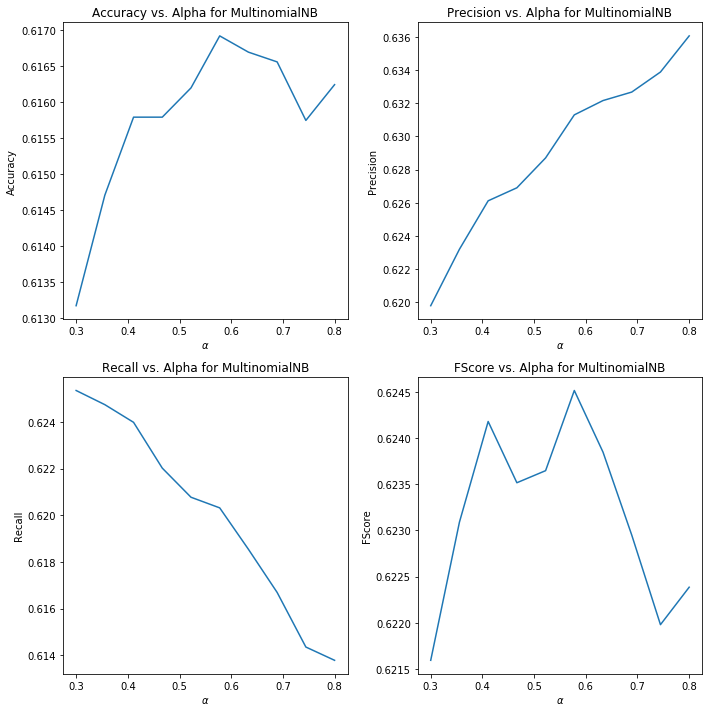
\includegraphics[width=\linewidth]{plots_nb.png}
		\caption{Naive Bayes (BOW)}
		\label{fig:nb_val}
	\end{subfigure}
	~
	% SVM (Word2Vec) validation
	\begin{subfigure}[h!]{0.3\textwidth}
		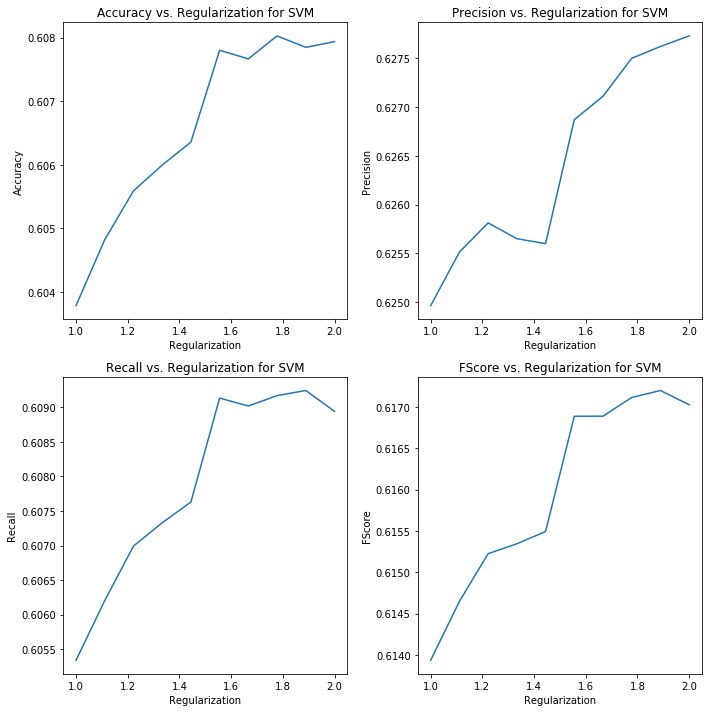
\includegraphics[width=\linewidth]{plots_svm1.png}
		\caption{SVM (Word2Vec)}
		\label{fig:svm1_val}
	\end{subfigure}
	~
	% SVM (Pre-trained Word2Vec) validation
	\begin{subfigure}[h!]{0.3\textwidth}
		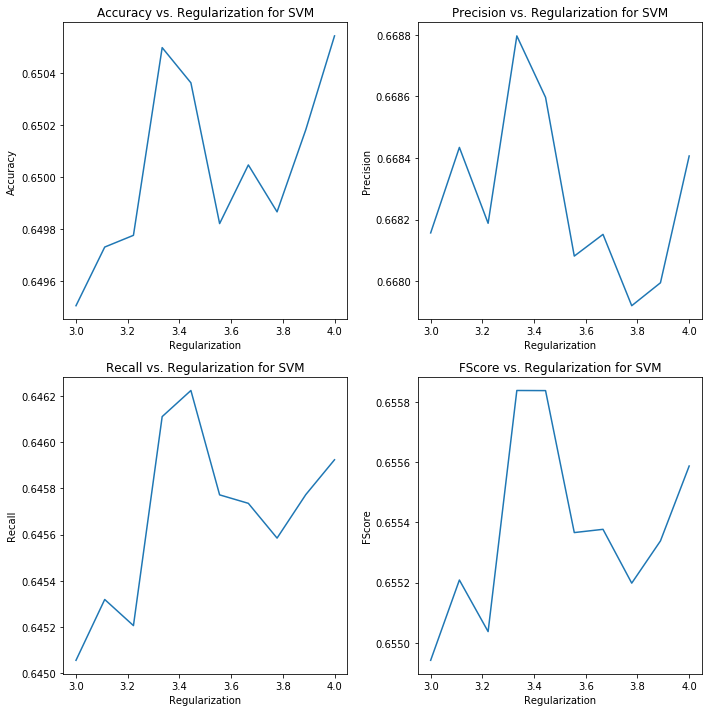
\includegraphics[width=\linewidth]{plots_svm2.png}
		\caption{SVM (Pre-trained Word2Vec)}
		\label{fig:svm2_val}
	\end{subfigure}
	\caption{Validation of models in ProTips}
	\label{fig:models_val}
\end{figure*}

% Final Measures
\begin{table*}[h!]
\centering
\begin{tabular}{|c|c|c|c|c|c|c|c|c|}
\hline
\rowcolor[HTML]{DDDDDD} 
\textbf{Repr.}                                                                                  & \textbf{Classifier}           & \textbf{Lapl.}       & \textbf{Reg.} & \textbf{Accuracy}       & \textbf{Avg.} & \textbf{Precision} & \textbf{Recall} & \textbf{FScore} \\ \hline
\cellcolor[HTML]{EFEFEF}                                                                                 &                               &                        &                         &                         & macro              & 0.64               & 0.64            & 0.64            \\ \cline{6-9} 
\multirow{-2}{*}{\cellcolor[HTML]{EFEFEF}BOW}                                                            & \multirow{-2}{*}{Naive Bayes} & \multirow{-2}{*}{0.58} & \multirow{-2}{*}{-}     & \multirow{-2}{*}{62.70\%} & micro              & 0.63               & 0.63            & 0.63            \\ \hline
\cellcolor[HTML]{EFEFEF}                                                                                 &                               &                        &                         &                         & macro              & 0.64               & 0.62            & 0.63            \\ \cline{6-9} 
\multirow{-2}{*}{\cellcolor[HTML]{EFEFEF}Word2Vec}                                                       & \multirow{-2}{*}{SVM}         & \multirow{-2}{*}{-}    & \multirow{-2}{*}{1.78}  & \multirow{-2}{*}{62.12\%} & micro              & 0.62               & 0.62            & 0.62            \\ \hline
\cellcolor[HTML]{EFEFEF}                                                                                 &                               &                        &                         &                         & macro              & 0.68                   & 0.65                & 0.66                \\ \cline{6-9} 
\multirow{-2}{*}{\cellcolor[HTML]{EFEFEF}\begin{tabular}[c]{@{}c@{}}Pre-trained\\ Word2Vec\end{tabular}} & \multirow{-2}{*}{SVM}         & \multirow{-2}{*}{-}    & \multirow{-2}{*}{4.00}  & \multirow{-2}{*}{65.79\%} & micro              & 0.66                   &               0.66  & 0.66                \\ \hline
\end{tabular}
\caption{Performance measures for employed methods in ProTips.}
\label{table:measures}
\end{table*}

% Conclusions
\section{Conclusions and further work}
\label{sec:conclusions}

% ProTips
In this paper an accuracy of $65.79\%$ was achieved for tip classification using SVM
and $300$D pre-trained word vectors. However, a Naive Bayes model was able to
achieve $62.70\%$ with a short training time, staying really close to SVM in precision,
recall and FScore. Thus, further exploration could show how
to improve the performance of BOW + Naive Bayes, or try to come up with better
language representations so that more complicated classifiers such as NNs
or SVMs can achieve higher performance and make the long training time worth it.\\
In either case, more data and processing power would be needed.

% Bibliography
\nocite{*}
\bibliography{acl2019}
\bibliographystyle{acl_natbib}

% Appendix
\appendix

\section{Other results}
\label{sec:other_results}
% PROTIPS
% Naive Bayes (BOW) Confusion Matrix
\begin{table*}[h!]
\centering
\begin{tabular}{c|c|c|c|c|}
\cline{2-5}
                                                            & \cellcolor[HTML]{EFEFEF}\textbf{Pred. ilpt} & \cellcolor[HTML]{EFEFEF}\textbf{Pred. lpt} & \cellcolor[HTML]{EFEFEF}\textbf{Pred. slpt} & \cellcolor[HTML]{EFEFEF}\textbf{Pred. ulpt} \\ \hline
\multicolumn{1}{|c|}{\cellcolor[HTML]{EFEFEF}\textbf{ilpt}} & 2280                                        & 124                                        & 213                                         & 704                                         \\ \hline
\multicolumn{1}{|c|}{\cellcolor[HTML]{EFEFEF}\textbf{lpt}}  & 347                                         & 6041                                       & 1871                                        & 1715                                        \\ \hline
\multicolumn{1}{|c|}{\cellcolor[HTML]{EFEFEF}\textbf{slpt}} & 198                                         & 1563                                       & 6059                                        & 2122                                        \\ \hline
\multicolumn{1}{|c|}{\cellcolor[HTML]{EFEFEF}\textbf{ulpt}} & 607                                         & 1085                                       & 1840                                        & 6443                                        \\ \hline
\end{tabular}
\caption{Confusion Matrix for Naive Bayes (BOW) in ProTips.}
\label{table:nb_cf}
\end{table*}

% SVM (Word2Vec) Confusion Matrix
\begin{table*}[h!]
\centering
\begin{tabular}{c|c|c|c|c|}
\cline{2-5}
                                                            & \cellcolor[HTML]{EFEFEF}\textbf{Pred. ilpt} & \cellcolor[HTML]{EFEFEF}\textbf{Pred. lpt} & \cellcolor[HTML]{EFEFEF}\textbf{Pred. slpt} & \cellcolor[HTML]{EFEFEF}\textbf{Pred. ulpt} \\ \hline
\multicolumn{1}{|c|}{\cellcolor[HTML]{EFEFEF}\textbf{ilpt}} & 2072                                        & 259                                        & 322                                         & 663                                         \\ \hline
\multicolumn{1}{|c|}{\cellcolor[HTML]{EFEFEF}\textbf{lpt}}  & 214                                         & 6649                                       & 1730                                        & 1391                                        \\ \hline
\multicolumn{1}{|c|}{\cellcolor[HTML]{EFEFEF}\textbf{slpt}} & 107                                         & 2058                                       & 5700                                        & 2071                                        \\ \hline
\multicolumn{1}{|c|}{\cellcolor[HTML]{EFEFEF}\textbf{ulpt}} & 427                                         & 1621                                       & 1714                                        & 6203                                        \\ \hline
\end{tabular}
\caption{Confusion Matrix for SVM (Word2Vec) in ProTips.}
\label{table:svm1_w2v}
\end{table*}

% SVM (Pre-trained Word2Vec) Confusion Matrix
\begin{table*}[h!]
\centering
\begin{tabular}{c|c|c|c|c|}
\cline{2-5}
                                                            & \cellcolor[HTML]{EFEFEF}\textbf{Pred. ilpt} & \cellcolor[HTML]{EFEFEF}\textbf{Pred. lpt} & \cellcolor[HTML]{EFEFEF}\textbf{Pred. slpt} & \cellcolor[HTML]{EFEFEF}\textbf{Pred. ulpt} \\ \hline
\multicolumn{1}{|c|}{\cellcolor[HTML]{EFEFEF}\textbf{ilpt}} & 2087                                        & 195                                        & 355                                         & 682                                         \\ \hline
\multicolumn{1}{|c|}{\cellcolor[HTML]{EFEFEF}\textbf{lpt}}  & 147                                         & 6966                                       & 1584                                        & 1283                                        \\ \hline
\multicolumn{1}{|c|}{\cellcolor[HTML]{EFEFEF}\textbf{slpt}} & 100                                         & 1766                                       & 6063                                        & 2006                                        \\ \hline
\multicolumn{1}{|c|}{\cellcolor[HTML]{EFEFEF}\textbf{ulpt}} & 394                                         & 1337                                       & 1511                                        & 6729                                        \\ \hline
\end{tabular}
\caption{Confusion Matrix for SVM (Pre-trained Word2Vec) in ProTips.}
\label{table:svm2_w2v}
\end{table*}

\end{document}